


\begin{document}
This report describes the design, construction, and analysis of an output stage for an operational ampifier. The topology chosen is two BJTs hooked together as shown in Figure \ref{fig:sample}.

\begin{figure}[H]
    \begin{center}
    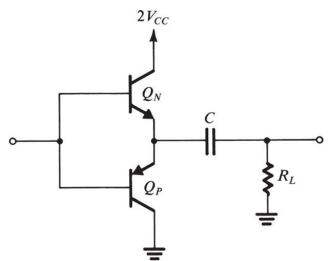
\includegraphics[scale=.45]{Introduction/outputstage.png}
    \caption{Sample single supply Class B output stage. \cite{b1}}
    \label{fig:sample}
    \end{center}
    
\end{figure}
Operational amplifiers serve an integral building block for modern electronics. Op amps provide large gain with various configuration schema. This allows the circuit designer to use the op amp in different topologies and achieve different results, all without modifying the op amp circuit itself. In addition, an op amp provides significant gain while maintaining stability, this is where the output stage comes in. The output stage allows design to accommodate for non-controllable factors such as transistor mismatch and temperature variation.   The objective of this lab is to create an op amp output stage out of discrete components that achieves the specifications as seen in Table \ref{tab:labspecs}.


\begin{table}[H]
\centering
\caption{Specifications}
\label{tab:labspecs}
\begin{tabular}{|l|l|}
\hline
\textbf{Specifications} &                 \\ \hline
Power                   & $\pm$5V         \\ \hline
Output Stage 			& $\geq$ 500$\Omega$ \\ \hline
Bias Current            & 400 $\mu$A      \\ \hline
Overall Voltage Gain    & $\geq$200V/V (46 dB)  \\ \hline
CMRR                    & $\geq$ 60dB     \\ \hline
Output Voltage Swing    & $\geq$ $\pm$ 2V \\ \hline
\end{tabular}
\end{table}

The application of negative feedback implies a 180$\deg$ phase shift. If the amplifier’s frequency response causes an additional 180$\deg$ phase shift, the feedback will add to the input signal instead of reducing it, which makes the op amp unstable if the amplifier’s gain is larger than unity at the same frequency. 

\noindent Section 2 of this report describes the design, and when relevant, the simulations of the experiments. Experimental results and implementation are addressed in Section 3, including reasoning as to why a different circuit than the one outlined previously was constructed. A discussion of the results, sources of error, and areas of possible improvement are outlined in Section 4. Section 5 concludes this report. \newline

\end{document}